\documentclass[twoside]{book}

% Packages required by doxygen
\usepackage{fixltx2e}
\usepackage{calc}
\usepackage{doxygen}
\usepackage[export]{adjustbox} % also loads graphicx
\usepackage{graphicx}
\usepackage[utf8]{inputenc}
\usepackage{makeidx}
\usepackage{multicol}
\usepackage{multirow}
\PassOptionsToPackage{warn}{textcomp}
\usepackage{textcomp}
\usepackage[nointegrals]{wasysym}
\usepackage[table]{xcolor}

% Font selection
\usepackage[T1]{fontenc}
\usepackage[scaled=.90]{helvet}
\usepackage{courier}
\usepackage{amssymb}
\usepackage{sectsty}
\renewcommand{\familydefault}{\sfdefault}
\allsectionsfont{%
  \fontseries{bc}\selectfont%
  \color{darkgray}%
}
\renewcommand{\DoxyLabelFont}{%
  \fontseries{bc}\selectfont%
  \color{darkgray}%
}
\newcommand{\+}{\discretionary{\mbox{\scriptsize$\hookleftarrow$}}{}{}}

% Page & text layout
\usepackage{geometry}
\geometry{%
  a4paper,%
  top=2.5cm,%
  bottom=2.5cm,%
  left=2.5cm,%
  right=2.5cm%
}
\tolerance=750
\hfuzz=15pt
\hbadness=750
\setlength{\emergencystretch}{15pt}
\setlength{\parindent}{0cm}
\setlength{\parskip}{3ex plus 2ex minus 2ex}
\makeatletter
\renewcommand{\paragraph}{%
  \@startsection{paragraph}{4}{0ex}{-1.0ex}{1.0ex}{%
    \normalfont\normalsize\bfseries\SS@parafont%
  }%
}
\renewcommand{\subparagraph}{%
  \@startsection{subparagraph}{5}{0ex}{-1.0ex}{1.0ex}{%
    \normalfont\normalsize\bfseries\SS@subparafont%
  }%
}
\makeatother

% Headers & footers
\usepackage{fancyhdr}
\pagestyle{fancyplain}
\fancyhead[LE]{\fancyplain{}{\bfseries\thepage}}
\fancyhead[CE]{\fancyplain{}{}}
\fancyhead[RE]{\fancyplain{}{\bfseries\leftmark}}
\fancyhead[LO]{\fancyplain{}{\bfseries\rightmark}}
\fancyhead[CO]{\fancyplain{}{}}
\fancyhead[RO]{\fancyplain{}{\bfseries\thepage}}
\fancyfoot[LE]{\fancyplain{}{}}
\fancyfoot[CE]{\fancyplain{}{}}
\fancyfoot[RE]{\fancyplain{}{\bfseries\scriptsize Generated by Doxygen }}
\fancyfoot[LO]{\fancyplain{}{\bfseries\scriptsize Generated by Doxygen }}
\fancyfoot[CO]{\fancyplain{}{}}
\fancyfoot[RO]{\fancyplain{}{}}
\renewcommand{\footrulewidth}{0.4pt}
\renewcommand{\chaptermark}[1]{%
  \markboth{#1}{}%
}
\renewcommand{\sectionmark}[1]{%
  \markright{\thesection\ #1}%
}

% Indices & bibliography
\usepackage{natbib}
\usepackage[titles]{tocloft}
\setcounter{tocdepth}{3}
\setcounter{secnumdepth}{5}
\makeindex

% Hyperlinks (required, but should be loaded last)
\usepackage{ifpdf}
\ifpdf
  \usepackage[pdftex,pagebackref=true]{hyperref}
\else
  \usepackage[ps2pdf,pagebackref=true]{hyperref}
\fi
\hypersetup{%
  colorlinks=true,%
  linkcolor=blue,%
  citecolor=blue,%
  unicode%
}

% Custom commands
\newcommand{\clearemptydoublepage}{%
  \newpage{\pagestyle{empty}\cleardoublepage}%
}

\usepackage{caption}
\captionsetup{labelsep=space,justification=centering,font={bf},singlelinecheck=off,skip=4pt,position=top}

%===== C O N T E N T S =====

\begin{document}

% Titlepage & ToC
\hypersetup{pageanchor=false,
             bookmarksnumbered=true,
             pdfencoding=unicode
            }
\pagenumbering{alph}
\begin{titlepage}
\vspace*{7cm}
\begin{center}%
{\Large My Project }\\
\vspace*{1cm}
{\large Generated by Doxygen 1.8.13}\\
\end{center}
\end{titlepage}
\clearemptydoublepage
\pagenumbering{roman}
\tableofcontents
\clearemptydoublepage
\pagenumbering{arabic}
\hypersetup{pageanchor=true}

%--- Begin generated contents ---
\chapter{assignment6}
\label{md___users_alexahong__desktop__fall__semester_2017-2018__c_s3560_homework_assignment6__r_e_a_d_m_e}
\Hypertarget{md___users_alexahong__desktop__fall__semester_2017-2018__c_s3560_homework_assignment6__r_e_a_d_m_e}
assignment 6\+: documentation tools in cs3560 
\chapter{Hierarchical Index}
\section{Class Hierarchy}
This inheritance list is sorted roughly, but not completely, alphabetically\+:\begin{DoxyCompactList}
\item \contentsline{section}{main\+\_\+savitch\+\_\+14\+:\+:game}{\pageref{classmain__savitch__14_1_1game}}{}
\begin{DoxyCompactList}
\item \contentsline{section}{main\+\_\+savitch\+\_\+14\+:\+:Othello}{\pageref{classmain__savitch__14_1_1_othello}}{}
\end{DoxyCompactList}
\item \contentsline{section}{piece}{\pageref{classpiece}}{}
\end{DoxyCompactList}

\chapter{Class Index}
\section{Class List}
Here are the classes, structs, unions and interfaces with brief descriptions\+:\begin{DoxyCompactList}
\item\contentsline{section}{\hyperlink{classmain__savitch__14_1_1game}{main\+\_\+savitch\+\_\+14\+::game} }{\pageref{classmain__savitch__14_1_1game}}{}
\item\contentsline{section}{\hyperlink{classmain__savitch__14_1_1Othello}{main\+\_\+savitch\+\_\+14\+::\+Othello} }{\pageref{classmain__savitch__14_1_1Othello}}{}
\item\contentsline{section}{\hyperlink{classpiece}{piece} }{\pageref{classpiece}}{}
\end{DoxyCompactList}

\chapter{File Index}
\section{File List}
Here is a list of all documented files with brief descriptions\+:\begin{DoxyCompactList}
\item\contentsline{section}{{\bfseries colors.\+h} }{\pageref{colors_8h}}{}
\item\contentsline{section}{\hyperlink{game_8cc}{game.\+cc} \\*Runs functions to play othello and determine whether its your move or the computer. Displays messages to the user and evlauates the AI potenial next move }{\pageref{game_8cc}}{}
\item\contentsline{section}{{\bfseries game.\+h} }{\pageref{game_8h}}{}
\item\contentsline{section}{\hyperlink{othello_8h}{othello.\+h} \\*This is the header file for othello that lets you play the game by keeping track of whose move it is letting you make moves and checking if theyre legal and checking if the game is over }{\pageref{othello_8h}}{}
\item\contentsline{section}{\hyperlink{piece_8h}{piece.\+h} \\*This file creates the peices for the game and checks if the pieces are the right color }{\pageref{piece_8h}}{}
\end{DoxyCompactList}

\chapter{Class Documentation}
\hypertarget{classmain__savitch__14_1_1game}{}\section{main\+\_\+savitch\+\_\+14\+:\+:game Class Reference}
\label{classmain__savitch__14_1_1game}\index{main\+\_\+savitch\+\_\+14\+::game@{main\+\_\+savitch\+\_\+14\+::game}}


Inheritance diagram for main\+\_\+savitch\+\_\+14\+:\+:game\+:
\nopagebreak
\begin{figure}[H]
\begin{center}
\leavevmode
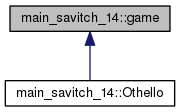
\includegraphics[width=207pt]{classmain__savitch__14_1_1game__inherit__graph}
\end{center}
\end{figure}
\subsection*{Public Types}
\begin{DoxyCompactItemize}
\item 
enum {\bfseries who} \{ {\bfseries H\+U\+M\+AN}, 
{\bfseries N\+E\+U\+T\+R\+AL}, 
{\bfseries C\+O\+M\+P\+U\+T\+ER}
 \}\hypertarget{classmain__savitch__14_1_1game_a4fe20fb287f809ae2b68e28e4ccba634}{}\label{classmain__savitch__14_1_1game_a4fe20fb287f809ae2b68e28e4ccba634}

\end{DoxyCompactItemize}
\subsection*{Public Member Functions}
\begin{DoxyCompactItemize}
\item 
who \hyperlink{classmain__savitch__14_1_1game_a4dbeaddb78059f7c5dcbf5cc4e026317}{play} ()
\begin{DoxyCompactList}\small\item\em The play function should not be overridden. It plays one round of the game, with the human player moving first and the computer second. The return value is the winner of the game (or N\+E\+U\+T\+R\+AL for a tie). \end{DoxyCompactList}\end{DoxyCompactItemize}
\subsection*{Protected Member Functions}
\begin{DoxyCompactItemize}
\item 
virtual void \hyperlink{classmain__savitch__14_1_1game_ab8b87c3a1b68634861a8c0ed2b9f1992}{display\+\_\+message} (const std\+::string \&message) const 
\begin{DoxyCompactList}\small\item\em displays string message to user. \end{DoxyCompactList}\item 
virtual std\+::string \hyperlink{classmain__savitch__14_1_1game_a1265f262f5a15bca5b532e6e97d13089}{get\+\_\+user\+\_\+move} () const 
\begin{DoxyCompactList}\small\item\em tells the user whos turn it is \end{DoxyCompactList}\item 
virtual who {\bfseries last\+\_\+mover} () const \hypertarget{classmain__savitch__14_1_1game_a38d435da6aadc192ac10160b26ea0cc1}{}\label{classmain__savitch__14_1_1game_a38d435da6aadc192ac10160b26ea0cc1}

\item 
virtual int {\bfseries moves\+\_\+completed} () const \hypertarget{classmain__savitch__14_1_1game_aee677d1ef52c35474cb7c6071bb71749}{}\label{classmain__savitch__14_1_1game_aee677d1ef52c35474cb7c6071bb71749}

\item 
virtual who {\bfseries next\+\_\+mover} () const \hypertarget{classmain__savitch__14_1_1game_a0d445fdec3201c91c145ee2763e08922}{}\label{classmain__savitch__14_1_1game_a0d445fdec3201c91c145ee2763e08922}

\item 
virtual who {\bfseries opposite} (who player) const \hypertarget{classmain__savitch__14_1_1game_ae38d001e92ebe46e1a1433e41446c7ab}{}\label{classmain__savitch__14_1_1game_ae38d001e92ebe46e1a1433e41446c7ab}

\item 
virtual void {\bfseries counting\+Pieces} ()=0\hypertarget{classmain__savitch__14_1_1game_a5954eccb6abf1ae900ad853ad2af99fa}{}\label{classmain__savitch__14_1_1game_a5954eccb6abf1ae900ad853ad2af99fa}

\item 
virtual void {\bfseries whos\+Turn} ()=0\hypertarget{classmain__savitch__14_1_1game_a98190a2bf784ce0f20533475754d136d}{}\label{classmain__savitch__14_1_1game_a98190a2bf784ce0f20533475754d136d}

\item 
virtual who \hyperlink{classmain__savitch__14_1_1game_a081611c42aa66b4d91bbefeec47c7c4e}{winning} () const 
\begin{DoxyCompactList}\small\item\em determines who is winning \end{DoxyCompactList}\item 
virtual void {\bfseries make\+\_\+move} (const std\+::string \&move)\hypertarget{classmain__savitch__14_1_1game_a20597d0caa907aea47b27fed8be3759b}{}\label{classmain__savitch__14_1_1game_a20597d0caa907aea47b27fed8be3759b}

\item 
virtual void {\bfseries restart} ()\hypertarget{classmain__savitch__14_1_1game_ad521a7d78e7c163a0bc28b709f0d45fd}{}\label{classmain__savitch__14_1_1game_ad521a7d78e7c163a0bc28b709f0d45fd}

\item 
virtual \hyperlink{classmain__savitch__14_1_1game}{game} $\ast$ {\bfseries clone} () const =0\hypertarget{classmain__savitch__14_1_1game_a7b663057f59210dd52738facfc40d959}{}\label{classmain__savitch__14_1_1game_a7b663057f59210dd52738facfc40d959}

\item 
virtual void {\bfseries compute\+\_\+moves} (std\+::queue$<$ std\+::string $>$ \&moves) const =0\hypertarget{classmain__savitch__14_1_1game_a2c0c049f5861026d0f639b5837889b7a}{}\label{classmain__savitch__14_1_1game_a2c0c049f5861026d0f639b5837889b7a}

\item 
virtual void {\bfseries display\+\_\+status} () const =0\hypertarget{classmain__savitch__14_1_1game_ac8205178922c49bab2865187e834b726}{}\label{classmain__savitch__14_1_1game_ac8205178922c49bab2865187e834b726}

\item 
virtual int {\bfseries evaluate} () const =0\hypertarget{classmain__savitch__14_1_1game_a9b9c8c5e9aa57c9a430f20b87cb047aa}{}\label{classmain__savitch__14_1_1game_a9b9c8c5e9aa57c9a430f20b87cb047aa}

\item 
virtual bool {\bfseries is\+\_\+game\+\_\+over} () const =0\hypertarget{classmain__savitch__14_1_1game_a49eed20648918b03fd3e2cf78987b3d1}{}\label{classmain__savitch__14_1_1game_a49eed20648918b03fd3e2cf78987b3d1}

\item 
virtual bool {\bfseries is\+\_\+legal} (const std\+::string \&move) const =0\hypertarget{classmain__savitch__14_1_1game_ad38351422ca1ee3ae58440c1c6b36b30}{}\label{classmain__savitch__14_1_1game_ad38351422ca1ee3ae58440c1c6b36b30}

\end{DoxyCompactItemize}
\subsection*{Protected Attributes}
\begin{DoxyCompactItemize}
\item 
int {\bfseries move\+\_\+number}\hypertarget{classmain__savitch__14_1_1game_ac4c296f4370d8e5bb5ea74b638fb827d}{}\label{classmain__savitch__14_1_1game_ac4c296f4370d8e5bb5ea74b638fb827d}

\end{DoxyCompactItemize}


\subsection{Member Function Documentation}
\index{main\+\_\+savitch\+\_\+14\+::game@{main\+\_\+savitch\+\_\+14\+::game}!display\+\_\+message@{display\+\_\+message}}
\index{display\+\_\+message@{display\+\_\+message}!main\+\_\+savitch\+\_\+14\+::game@{main\+\_\+savitch\+\_\+14\+::game}}
\subsubsection[{\texorpdfstring{display\+\_\+message(const std\+::string \&message) const }{display_message(const std::string &message) const }}]{\setlength{\rightskip}{0pt plus 5cm}void main\+\_\+savitch\+\_\+14\+::game\+::display\+\_\+message (
\begin{DoxyParamCaption}
\item[{const std\+::string \&}]{message}
\end{DoxyParamCaption}
) const\hspace{0.3cm}{\ttfamily [protected]}, {\ttfamily [virtual]}}\hypertarget{classmain__savitch__14_1_1game_ab8b87c3a1b68634861a8c0ed2b9f1992}{}\label{classmain__savitch__14_1_1game_ab8b87c3a1b68634861a8c0ed2b9f1992}


displays string message to user. 


\begin{DoxyParams}{Parameters}
{\em message} & -\/ the message that will be displayed to user \\
\hline
\end{DoxyParams}
\begin{DoxyReturn}{Returns}
void 
\end{DoxyReturn}
\index{main\+\_\+savitch\+\_\+14\+::game@{main\+\_\+savitch\+\_\+14\+::game}!get\+\_\+user\+\_\+move@{get\+\_\+user\+\_\+move}}
\index{get\+\_\+user\+\_\+move@{get\+\_\+user\+\_\+move}!main\+\_\+savitch\+\_\+14\+::game@{main\+\_\+savitch\+\_\+14\+::game}}
\subsubsection[{\texorpdfstring{get\+\_\+user\+\_\+move() const }{get_user_move() const }}]{\setlength{\rightskip}{0pt plus 5cm}string main\+\_\+savitch\+\_\+14\+::game\+::get\+\_\+user\+\_\+move (
\begin{DoxyParamCaption}
{}
\end{DoxyParamCaption}
) const\hspace{0.3cm}{\ttfamily [protected]}, {\ttfamily [virtual]}}\hypertarget{classmain__savitch__14_1_1game_a1265f262f5a15bca5b532e6e97d13089}{}\label{classmain__savitch__14_1_1game_a1265f262f5a15bca5b532e6e97d13089}


tells the user whos turn it is 

\begin{DoxyReturn}{Returns}
answer, a string 
\end{DoxyReturn}
\index{main\+\_\+savitch\+\_\+14\+::game@{main\+\_\+savitch\+\_\+14\+::game}!play@{play}}
\index{play@{play}!main\+\_\+savitch\+\_\+14\+::game@{main\+\_\+savitch\+\_\+14\+::game}}
\subsubsection[{\texorpdfstring{play()}{play()}}]{\setlength{\rightskip}{0pt plus 5cm}game\+::who main\+\_\+savitch\+\_\+14\+::game\+::play (
\begin{DoxyParamCaption}
{}
\end{DoxyParamCaption}
)}\hypertarget{classmain__savitch__14_1_1game_a4dbeaddb78059f7c5dcbf5cc4e026317}{}\label{classmain__savitch__14_1_1game_a4dbeaddb78059f7c5dcbf5cc4e026317}


The play function should not be overridden. It plays one round of the game, with the human player moving first and the computer second. The return value is the winner of the game (or N\+E\+U\+T\+R\+AL for a tie). 

\begin{DoxyReturn}{Returns}
H\+U\+M\+AN player 
\end{DoxyReturn}
\index{main\+\_\+savitch\+\_\+14\+::game@{main\+\_\+savitch\+\_\+14\+::game}!winning@{winning}}
\index{winning@{winning}!main\+\_\+savitch\+\_\+14\+::game@{main\+\_\+savitch\+\_\+14\+::game}}
\subsubsection[{\texorpdfstring{winning() const }{winning() const }}]{\setlength{\rightskip}{0pt plus 5cm}game\+::who main\+\_\+savitch\+\_\+14\+::game\+::winning (
\begin{DoxyParamCaption}
{}
\end{DoxyParamCaption}
) const\hspace{0.3cm}{\ttfamily [protected]}, {\ttfamily [virtual]}}\hypertarget{classmain__savitch__14_1_1game_a081611c42aa66b4d91bbefeec47c7c4e}{}\label{classmain__savitch__14_1_1game_a081611c42aa66b4d91bbefeec47c7c4e}


determines who is winning 

\begin{DoxyReturn}{Returns}
determines who is winning or if they have the same score. 
\end{DoxyReturn}


Reimplemented in \hyperlink{classmain__savitch__14_1_1Othello_a8934d1b63f73c03dae9629dbe03955d7}{main\+\_\+savitch\+\_\+14\+::\+Othello}.



The documentation for this class was generated from the following files\+:\begin{DoxyCompactItemize}
\item 
game.\+h\item 
\hyperlink{game_8cc}{game.\+cc}\end{DoxyCompactItemize}

\hypertarget{classmain__savitch__14_1_1_othello}{}\section{main\+\_\+savitch\+\_\+14\+:\+:Othello Class Reference}
\label{classmain__savitch__14_1_1_othello}\index{main\+\_\+savitch\+\_\+14\+::\+Othello@{main\+\_\+savitch\+\_\+14\+::\+Othello}}
Inheritance diagram for main\+\_\+savitch\+\_\+14\+:\+:Othello\+:\begin{figure}[H]
\begin{center}
\leavevmode
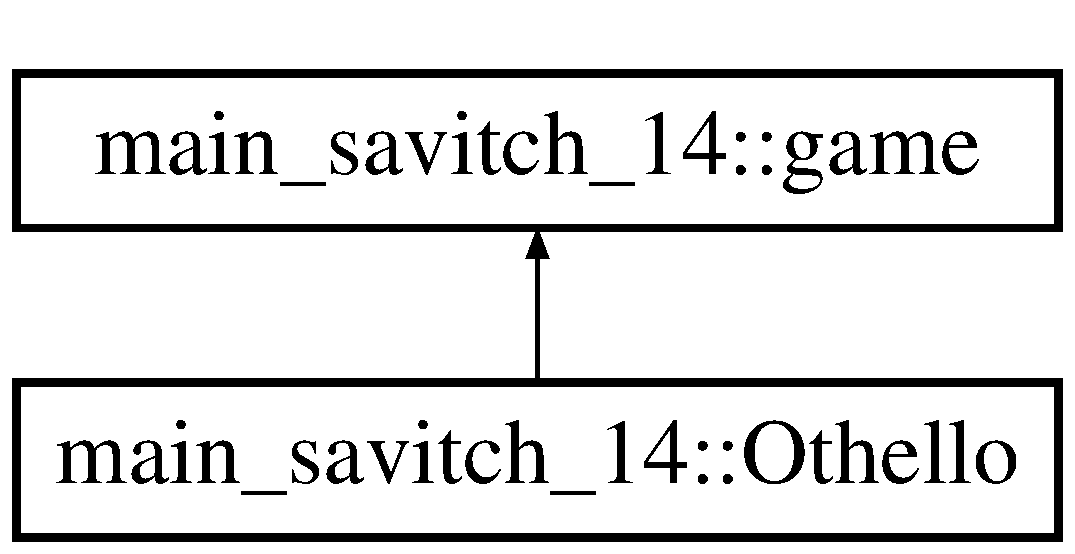
\includegraphics[height=2.000000cm]{classmain__savitch__14_1_1_othello}
\end{center}
\end{figure}
\subsection*{Public Member Functions}
\begin{DoxyCompactItemize}
\item 
\mbox{\Hypertarget{classmain__savitch__14_1_1_othello_ab01a4f7aba130133221a11224905e8ce}\label{classmain__savitch__14_1_1_othello_ab01a4f7aba130133221a11224905e8ce}} 
void {\bfseries display\+\_\+status} () const
\item 
\mbox{\Hypertarget{classmain__savitch__14_1_1_othello_a57ae44590de8d683592f186ed6bd25b0}\label{classmain__savitch__14_1_1_othello_a57ae44590de8d683592f186ed6bd25b0}} 
int {\bfseries evaluate} () const
\item 
bool \hyperlink{classmain__savitch__14_1_1_othello_a540c8b0030e429e0ac30f07e9e8868ec}{is\+\_\+game\+\_\+over} () const
\begin{DoxyCompactList}\small\item\em this function checks if the game is over \end{DoxyCompactList}\item 
\mbox{\Hypertarget{classmain__savitch__14_1_1_othello_a74ac0d4e6399167037dfc708efdb9033}\label{classmain__savitch__14_1_1_othello_a74ac0d4e6399167037dfc708efdb9033}} 
bool {\bfseries is\+\_\+legal} (const string \&move) const
\item 
\mbox{\Hypertarget{classmain__savitch__14_1_1_othello_a1066b280efa5cb41039585669282fe06}\label{classmain__savitch__14_1_1_othello_a1066b280efa5cb41039585669282fe06}} 
void {\bfseries make\+\_\+move} (const string \&move)
\item 
\mbox{\Hypertarget{classmain__savitch__14_1_1_othello_abf872b8074bfa4c04119317dc3b39af2}\label{classmain__savitch__14_1_1_othello_abf872b8074bfa4c04119317dc3b39af2}} 
void {\bfseries restart} ()
\item 
\mbox{\Hypertarget{classmain__savitch__14_1_1_othello_a3177234195a490eef52343d957e64b5d}\label{classmain__savitch__14_1_1_othello_a3177234195a490eef52343d957e64b5d}} 
void {\bfseries make\+\_\+skips} ()
\item 
\mbox{\Hypertarget{classmain__savitch__14_1_1_othello_a19f49edfbe82b84922877e00bc854ed8}\label{classmain__savitch__14_1_1_othello_a19f49edfbe82b84922877e00bc854ed8}} 
void {\bfseries counting\+Pieces} ()
\item 
\mbox{\Hypertarget{classmain__savitch__14_1_1_othello_a21440dbb4511812a76c578a5f546710b}\label{classmain__savitch__14_1_1_othello_a21440dbb4511812a76c578a5f546710b}} 
void {\bfseries whos\+Turn} ()
\item 
\mbox{\Hypertarget{classmain__savitch__14_1_1_othello_a7a5f8495f1a61f6e7b3968e919013c18}\label{classmain__savitch__14_1_1_othello_a7a5f8495f1a61f6e7b3968e919013c18}} 
\hyperlink{classmain__savitch__14_1_1game}{game} $\ast$ {\bfseries clone} () const
\item 
\mbox{\Hypertarget{classmain__savitch__14_1_1_othello_a921d4ffa277b0250f187f20b9598ebb1}\label{classmain__savitch__14_1_1_othello_a921d4ffa277b0250f187f20b9598ebb1}} 
void {\bfseries compute\+\_\+moves} (std\+::queue$<$ std\+::string $>$ \&moves) const
\item 
who \hyperlink{classmain__savitch__14_1_1_othello_a4ea78b18eea66c944c0a9356349e0fd4}{winning} () const
\begin{DoxyCompactList}\small\item\em determines who is winning \end{DoxyCompactList}\end{DoxyCompactItemize}
\subsection*{Protected Attributes}
\begin{DoxyCompactItemize}
\item 
\mbox{\Hypertarget{classmain__savitch__14_1_1_othello_a2eed818925f68d5678b78107a3298138}\label{classmain__savitch__14_1_1_othello_a2eed818925f68d5678b78107a3298138}} 
int {\bfseries black}
\item 
\mbox{\Hypertarget{classmain__savitch__14_1_1_othello_a7d5f59b1e581ed7a8145debeecf4f310}\label{classmain__savitch__14_1_1_othello_a7d5f59b1e581ed7a8145debeecf4f310}} 
int {\bfseries white}
\item 
\mbox{\Hypertarget{classmain__savitch__14_1_1_othello_a85d4ce17512d8dbf85a313a27eea0644}\label{classmain__savitch__14_1_1_othello_a85d4ce17512d8dbf85a313a27eea0644}} 
int {\bfseries skips}
\item 
\mbox{\Hypertarget{classmain__savitch__14_1_1_othello_a15045e3e94c34afe08240885e230d502}\label{classmain__savitch__14_1_1_othello_a15045e3e94c34afe08240885e230d502}} 
int {\bfseries open\+Spots}
\item 
\mbox{\Hypertarget{classmain__savitch__14_1_1_othello_a98fbc46241d2f5e05ccb4b66f11535bf}\label{classmain__savitch__14_1_1_othello_a98fbc46241d2f5e05ccb4b66f11535bf}} 
int {\bfseries b}
\item 
\mbox{\Hypertarget{classmain__savitch__14_1_1_othello_a1b11c5fe33e30a94ed39e8cb55caf37e}\label{classmain__savitch__14_1_1_othello_a1b11c5fe33e30a94ed39e8cb55caf37e}} 
int {\bfseries w}
\end{DoxyCompactItemize}
\subsection*{Additional Inherited Members}


\subsection{Member Function Documentation}
\mbox{\Hypertarget{classmain__savitch__14_1_1_othello_a540c8b0030e429e0ac30f07e9e8868ec}\label{classmain__savitch__14_1_1_othello_a540c8b0030e429e0ac30f07e9e8868ec}} 
\index{main\+\_\+savitch\+\_\+14\+::\+Othello@{main\+\_\+savitch\+\_\+14\+::\+Othello}!is\+\_\+game\+\_\+over@{is\+\_\+game\+\_\+over}}
\index{is\+\_\+game\+\_\+over@{is\+\_\+game\+\_\+over}!main\+\_\+savitch\+\_\+14\+::\+Othello@{main\+\_\+savitch\+\_\+14\+::\+Othello}}
\subsubsection{\texorpdfstring{is\+\_\+game\+\_\+over()}{is\_game\_over()}}
{\footnotesize\ttfamily bool main\+\_\+savitch\+\_\+14\+::\+Othello\+::is\+\_\+game\+\_\+over (\begin{DoxyParamCaption}{ }\end{DoxyParamCaption}) const\hspace{0.3cm}{\ttfamily [virtual]}}



this function checks if the game is over 

\begin{DoxyReturn}{Returns}
bool 
\end{DoxyReturn}


Implements \hyperlink{classmain__savitch__14_1_1game}{main\+\_\+savitch\+\_\+14\+::game}.

\mbox{\Hypertarget{classmain__savitch__14_1_1_othello_a4ea78b18eea66c944c0a9356349e0fd4}\label{classmain__savitch__14_1_1_othello_a4ea78b18eea66c944c0a9356349e0fd4}} 
\index{main\+\_\+savitch\+\_\+14\+::\+Othello@{main\+\_\+savitch\+\_\+14\+::\+Othello}!winning@{winning}}
\index{winning@{winning}!main\+\_\+savitch\+\_\+14\+::\+Othello@{main\+\_\+savitch\+\_\+14\+::\+Othello}}
\subsubsection{\texorpdfstring{winning()}{winning()}}
{\footnotesize\ttfamily game\+::who main\+\_\+savitch\+\_\+14\+::\+Othello\+::winning (\begin{DoxyParamCaption}{ }\end{DoxyParamCaption}) const\hspace{0.3cm}{\ttfamily [virtual]}}



determines who is winning 

\begin{DoxyReturn}{Returns}
determines who is winning or if they have the same score. 
\end{DoxyReturn}


Reimplemented from \hyperlink{classmain__savitch__14_1_1game_a2f0d5338c12bd98d52fe2383ece5c45e}{main\+\_\+savitch\+\_\+14\+::game}.



The documentation for this class was generated from the following files\+:\begin{DoxyCompactItemize}
\item 
/\+Users/alexahong/\+Desktop/\+Fall Semester 2017-\/2018/\+C\+S3560/homework/assignment6/\hyperlink{othello_8h}{othello.\+h}\item 
/\+Users/alexahong/\+Desktop/\+Fall Semester 2017-\/2018/\+C\+S3560/homework/assignment6/othello.\+cc\end{DoxyCompactItemize}

\hypertarget{classpiece}{}\section{piece Class Reference}
\label{classpiece}\index{piece@{piece}}
\subsection*{Public Member Functions}
\begin{DoxyCompactItemize}
\item 
void \hyperlink{classpiece_ab898c5827a5859e4cddc9d61a814a873}{flip} ()
\begin{DoxyCompactList}\small\item\em this function flips the piece to the opposite color \end{DoxyCompactList}\item 
bool {\bfseries is\+\_\+blank} () const \hypertarget{classpiece_af8e5afd9e1eb6b367c7da643c94c7113}{}\label{classpiece_af8e5afd9e1eb6b367c7da643c94c7113}

\item 
bool {\bfseries is\+\_\+black} () const \hypertarget{classpiece_abb229bd7452561f1f3aa794e5561aa60}{}\label{classpiece_abb229bd7452561f1f3aa794e5561aa60}

\item 
bool {\bfseries is\+\_\+white} () const \hypertarget{classpiece_a229a0c4b29e449350b2c3ba019e6c9a9}{}\label{classpiece_a229a0c4b29e449350b2c3ba019e6c9a9}

\item 
void \hyperlink{classpiece_a31480899f2a591fdb22d97933303e19d}{set\+\_\+white} ()
\begin{DoxyCompactList}\small\item\em this function sets the color of a piece to white \end{DoxyCompactList}\item 
void {\bfseries set\+\_\+black} ()\hypertarget{classpiece_a273d63d07b6ea973b2fc4f7e1b56ea10}{}\label{classpiece_a273d63d07b6ea973b2fc4f7e1b56ea10}

\end{DoxyCompactItemize}


\subsection{Member Function Documentation}
\index{piece@{piece}!flip@{flip}}
\index{flip@{flip}!piece@{piece}}
\subsubsection[{\texorpdfstring{flip()}{flip()}}]{\setlength{\rightskip}{0pt plus 5cm}void piece\+::flip (
\begin{DoxyParamCaption}
{}
\end{DoxyParamCaption}
)\hspace{0.3cm}{\ttfamily [inline]}}\hypertarget{classpiece_ab898c5827a5859e4cddc9d61a814a873}{}\label{classpiece_ab898c5827a5859e4cddc9d61a814a873}


this function flips the piece to the opposite color 

\begin{DoxyReturn}{Returns}
void 
\end{DoxyReturn}
\index{piece@{piece}!set\+\_\+white@{set\+\_\+white}}
\index{set\+\_\+white@{set\+\_\+white}!piece@{piece}}
\subsubsection[{\texorpdfstring{set\+\_\+white()}{set_white()}}]{\setlength{\rightskip}{0pt plus 5cm}void piece\+::set\+\_\+white (
\begin{DoxyParamCaption}
{}
\end{DoxyParamCaption}
)\hspace{0.3cm}{\ttfamily [inline]}}\hypertarget{classpiece_a31480899f2a591fdb22d97933303e19d}{}\label{classpiece_a31480899f2a591fdb22d97933303e19d}


this function sets the color of a piece to white 

\begin{DoxyReturn}{Returns}
void 
\end{DoxyReturn}


The documentation for this class was generated from the following file\+:\begin{DoxyCompactItemize}
\item 
\hyperlink{piece_8h}{piece.\+h}\end{DoxyCompactItemize}

\chapter{File Documentation}
\hypertarget{game_8cc}{}\section{/\+Users/alexahong/\+Desktop/\+Fall Semester 2017-\/2018/\+C\+S3560/homework/assignment6/game.cc File Reference}
\label{game_8cc}\index{/\+Users/alexahong/\+Desktop/\+Fall Semester 2017-\/2018/\+C\+S3560/homework/assignment6/game.\+cc@{/\+Users/alexahong/\+Desktop/\+Fall Semester 2017-\/2018/\+C\+S3560/homework/assignment6/game.\+cc}}


runs functions to play othello and determine whether its your move or the computer. Displays messages to the user and evlauates the AI potenial next move.  


{\ttfamily \#include $<$cassert$>$}\newline
{\ttfamily \#include $<$climits$>$}\newline
{\ttfamily \#include $<$iostream$>$}\newline
{\ttfamily \#include $<$queue$>$}\newline
{\ttfamily \#include $<$string$>$}\newline
{\ttfamily \#include \char`\"{}game.\+h\char`\"{}}\newline


\subsection{Detailed Description}
runs functions to play othello and determine whether its your move or the computer. Displays messages to the user and evlauates the AI potenial next move. 


\hypertarget{othello_8h}{}\section{/\+Users/alexahong/\+Desktop/\+Fall Semester 2017-\/2018/\+C\+S3560/homework/assignment6/othello.h File Reference}
\label{othello_8h}\index{/\+Users/alexahong/\+Desktop/\+Fall Semester 2017-\/2018/\+C\+S3560/homework/assignment6/othello.\+h@{/\+Users/alexahong/\+Desktop/\+Fall Semester 2017-\/2018/\+C\+S3560/homework/assignment6/othello.\+h}}


This is the header file for othello that lets you play the game by keeping track of whose move it is letting you make moves and checking if theyre legal and checking if the game is over.  


{\ttfamily \#include \char`\"{}game.\+h\char`\"{}}\newline
{\ttfamily \#include \char`\"{}piece.\+h\char`\"{}}\newline
{\ttfamily \#include \char`\"{}colors.\+h\char`\"{}}\newline
{\ttfamily \#include $<$iostream$>$}\newline
\subsection*{Classes}
\begin{DoxyCompactItemize}
\item 
class \hyperlink{classmain__savitch__14_1_1_othello}{main\+\_\+savitch\+\_\+14\+::\+Othello}
\end{DoxyCompactItemize}


\subsection{Detailed Description}
This is the header file for othello that lets you play the game by keeping track of whose move it is letting you make moves and checking if theyre legal and checking if the game is over. 


\hypertarget{piece_8h}{}\section{piece.\+h File Reference}
\label{piece_8h}\index{piece.\+h@{piece.\+h}}


this file creates the peices for the game and checks if the pieces are the right color  


This graph shows which files directly or indirectly include this file\+:
\nopagebreak
\begin{figure}[H]
\begin{center}
\leavevmode
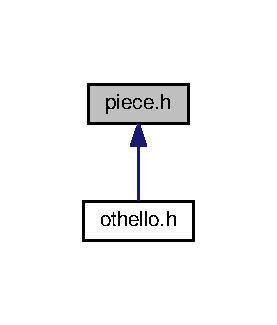
\includegraphics[width=133pt]{piece_8h__dep__incl}
\end{center}
\end{figure}
\subsection*{Classes}
\begin{DoxyCompactItemize}
\item 
class \hyperlink{classpiece}{piece}
\end{DoxyCompactItemize}
\subsection*{Enumerations}
\begin{DoxyCompactItemize}
\item 
enum {\bfseries color} \{ {\bfseries black}, 
{\bfseries white}, 
{\bfseries blank}
 \}\hypertarget{piece_8h_a37dbdc30935031c05304482e1be89d8f}{}\label{piece_8h_a37dbdc30935031c05304482e1be89d8f}

\end{DoxyCompactItemize}


\subsection{Detailed Description}
this file creates the peices for the game and checks if the pieces are the right color 


%--- End generated contents ---

% Index
\backmatter
\newpage
\phantomsection
\clearemptydoublepage
\addcontentsline{toc}{chapter}{Index}
\printindex

\end{document}
